\documentclass[../main.tex]{subfiles}

\begin{document}

%%%%%%%%%%%%%%%%%%%%%%%%%%%%%%%%%%%%%%%%%%%%%%%%%%%%%%%%%%%%%%%%%%%%%%%%%%%%%%%%%%%%%%%%%%%%%%%%%%%%%%%%%
\section{Stejnoměrná spojitost}
%%%%%%%%%%%%%%%%%%%%%%%%%%%%%%%%%%%%%%%%%%%%%%%%%%%%%%%%%%%%%%%%%%%%%%%%%%%%%%%%%%%%%%%%%%%%%%%%%%%%%%%%%
\begin{definition}[Stejnoměrná spojitost]
	Řekneme, že $f : (X,d) \rightarrow (Y,d')$ je stejnoměrně spojitá, pokud
	\[\forall \varepsilon > 0 \exists \delta > 0 : \forall x,y : d(x,y) < \delta \implies d'(f(x),f(y)) < \varepsilon\]
\end{definition}

\begin{intuition}
	Geometrický význam je ten, že pro libovolnou vzdálenost \(\varepsilon\) v \(y\) existuje \(\delta\) t. ž. okénko o velikosti \((\delta, \varepsilon)\) umístěné do libovolného místa v grafu není grafem protnuto nahoře ani dole. Na obrázku \ref{fig:con} je vidět, že funkce \(\sqrt{x}\) stejnosměrnou spojitost splňuje, kdežto funkce \(\frac{1}{x}\) nikoliv.

	\begin{figure}[h]
		\centering
		\subfloat{{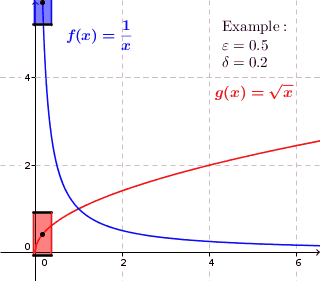
\includegraphics[width=4cm]{07-1}}}%
		\hspace{3em}
		\subfloat{{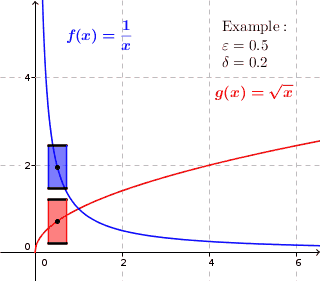
\includegraphics[width=4cm]{07-2}}}%
		\hspace{3em}
		\subfloat{{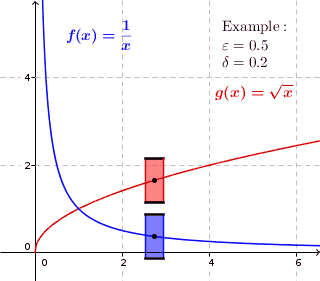
\includegraphics[width=4cm]{07-3}}}%
		\caption{Geometrický význam stejnosměrné spojitosti pro \(f(x) = 1/x\) a \(g(x) = \sqrt{x}\) na intervalu \(\mathbb{R}^+\).}
		\label{fig:con}
	\end{figure}

	V porovnání s definicí normální spojitosti je rozdíl v pozici kvantifikátorů \(\forall x, y\) (v definici spojitosti jsou na úplném začátku). To odpovídá tomu, že pro spojitost požadujeme okénko pouze \textbf{pro jeden bod} a ne pro celou funkci, jak je tomu u stejnoměrné spojitosti.
\end{intuition}

\begin{theorem}[Spojitost zobrazení na kompaktním prostoru]
	Je-li $(X,d)$ kompaktní, je každé spojité $f : (X,d) \rightarrow (Y,d')$ stejnoměrně spojité. Zejména to platí 
	pro spojité reálné funkce na kompaktních intervalech.
\end{theorem}

\begin{proof}
	Nechť $f : (X,d) \rightarrow (Y,d')$ není stejnoměrně spojité. Potom $\exists \varepsilon > 0 : \forall n\ \exists x_n, y_n :$
	\[d(x_n,y_n) < \frac{1}{n}\]
	ale
	\[d'(f(x_n),f(y_n)) \geq \varepsilon.\]
	Zvolme konvergentní podposloupnost $(x_{k_n})_n$ posloupnosti $(x_n)_n$. Označme $a = \lim_n x_{k_n}.$ Potom podle $d(x_n,y_n) < \frac{1}{n}$ je též 
	$a = \lim_n y_{k_n}.$ Podle $d'(f(x_n),f(y_n)) \geq \varepsilon$ nemůže být $f(a) = \lim_n f(x_{k_n})$ a zároveň $f(a) = \lim_n f(y_{k_n})$, 
	a tedy $f$ není ani spojité.
\end{proof}

\end{document}
